\chapter{Design}
The network forensics is the field of digital forensics in computer networks.
The objective is to monitor and anaylse the network traffic for the purpose of dealing with the network crimes.
Network forensics is defined as “the use of scientifically
proven techniques to collect, fuse, identify, examine, correlate, analyze, and document digital evidence from multiple, actively processing and transmitting digital sources for the purpose of uncovering facts related to the planned intent, or measured success of unauthorized activities meant to disrupt, corrupt, and or compromise system components as well as providing information to assist in response to or recovery from these activities” \cite{palmer2001road}.
The proposed network forensic system consists of a capture module, anaylsis module and visualization module.
The system is designed to capture the network traffic from the different hosts in the internet, categorize the port scanning packets, analyse it and visualise the needed information.
The capture module consists of a network telescope and a place to store the captured packets.
The purpose of the anaylsis module is to separate the port  scanning packets from other illegitimate packets.
The illegitimate packets can be denial-of-service attacks, Internet worms, malicious network scans or due to misconfiguration problems.\\\\ 
The suggested network forensics system which is designed to monitor the port scanning activities is shown in the Figure 4.1.
It consists of mainly three modules: capture module, analysis module and visualization module.
The capture module includes network telescope which is dedicated for capturing the IPv4 packets.
Each packet goes through the capture module and store it in hard disk.
The analysis module analyses each packet from the hard disk and decide whether it is port scanning packet or not. 
Afterwards it separates the port scanning packets from other illegitimate packets.
The visualization module uses the port scanning packets and provide the valuable information about the behavior of the port scanning.
\begin{figure}[t]
    \centering
	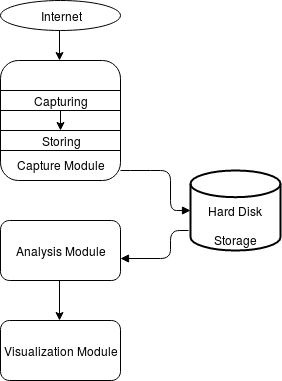
\includegraphics[width=7cm, height=8cm]{images/networkforensic_arch}
	\caption{ The Architecture of Network Forensic System}
\end{figure}
\section{Capture Module}
The primary task of the capture module is to capture the network 
activity that is capable of network attack.
This module can be subdivided into two sub modules: capturing and storing.
\subsection{Capturing}
\begin{figure}[t]
    \centering
	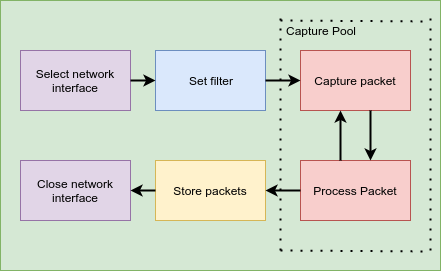
\includegraphics[width=10cm, height=6cm]{images/packetcapture_flow1.png}
	\caption{ Program Flow of Packet Capturing System}
\end{figure}
This module contains network telescope which capture all the incoming packets passing through the network interface of the host.
Network telescope is associated with packet capturing system, which actually does the work of collecting the packets that pass through a given network interface.
Packet capturing system is designed for UNIX system based on libpcap, an open source library that provides a high level interface to network packet capture systems.\\\\
Figure 4.2 shows the important steps in the  the packet capturing system.
Initially we need to select the network interface to listen on.
When the kernel gets a packet from the network interface, it has to copy the packet from kernel space to user space. 
Performing this task on every packet will reduce the performance of our packet capturing system and kernel may drop packets.
To counter this problem, we set a filter to avoid capturing packets from server address, thus capture packets only from  specific range of IP addresses.
After setting up a filter expression, we start capturing the packets and  dissect packet into different headers and process it.
These processed packets are stored in a separate file in the next step.
Once we decide to stop capturing process, we close the interface and exit from the capturing procedure.\\\\
The packet capturing process take place in two stages. 
In the first stage, the network telescope is designed as active in such a way that it does not send anything unless it receives a request. 
In the second stage, the network telescope is associated with T-Pot, a multi-honeypot platform system from Deutsche Telekom.
Network telescope configuration at these two phases will be explained in detail in Chapter 5.
\subsection{Storing}
Storage and processing are also significant aspects to consider, as traffic that has been captured needs to be stored somewhere for further analysis.
This module stores the captured packets to the hard disk of the host system, in order to do the further investigation on the packets.
Once the packets have been collected, storage provision needs to be made to store the packets.
Due to the limited size of the hard disk, we used the logrotate command to rotate the logfiles on weekly basis.
The UNIX logrotate utility can be used to rotate the log files when size of the file reaches a certain level.\\\\
These packets were stored in pcap file format which is a basic and common method to store captured network data.
We decided to store the packets in pcap format because of its immense popularity in network packet capture and exchange formats.
Pcap format is defined by libpcap, a portable C/C++ library for network traffic capture for UNIX systems.
Moreover popular networking tools such as tcpdump, Wireshark, libtrace, tcpsplice use pcap file format to capture and process the packets.
\section{Analysis Module}
\begin{figure}[t]
\centering
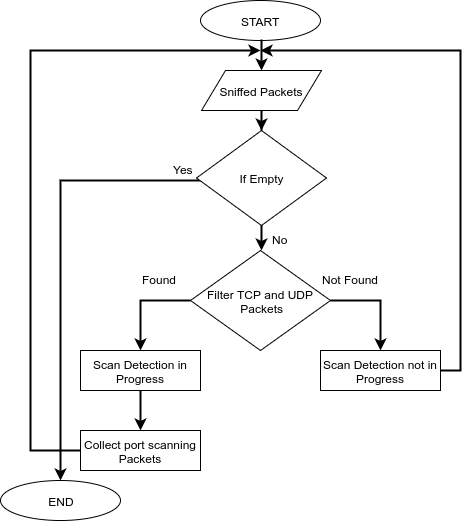
\includegraphics[width=8cm, height=10cm]{images/analysis_flow.png}
\caption{ The Data Flow Diagram of Port Scan Detection}
\end{figure}
The analysis module analyses the captured files stored in the system by the capture module, with a specific end goal to find the behavior and source of the  port scanning attack.
In order to do that, it is important to separate the port scanning packets from other malicious traffic.\\\\
The port scanning detection mechanism is basically designed  to detect TCP and UDP scans.
In addition to that, it divides port scanning activities into different categories.
The port scans can be divided into mainly two types based on the pattern of 
destination ports and target destinations the scan examines: vertical and horizontal scans.
The vertical scan is a port scan which targets multiple destination ports on a same IP address.
This is one among the easiest one to detect because only one host needs to be investigated. 
The horizontal scan is a port scan which scans multiple IP addresses, but targets only one specific port.
However Internet scanners provide several methods to hide the port scanning activity from the host system, thus avoiding the detection of port scanning mechanisms as explained in the Section 2.2.2.
One method to avoid the detection is to increase the timing between two successive scans in the same network or host.
In order to tackle this problem, we design our algorithm in such a way that it look for port scans from the same source for a definite amount of time. 
Another method to evade the detection is to scan from a block of addresses using spoofed IP or IP decoys.
We try to quantify this error using two methods.
Initially, we design an approach to minimize the false positives in the result by just combining the IPs from the same /24 network which target the same set of hosts and ports \cite{lee2003detection}.
The second method is a tentative approach to  minimize the error, by considering that possibly all attacks from same source come from the same Internet Service Provider (ISP).\\\\ 
Furthermore the port scanning activity can be divided based on the techniques users apply to scan the network.
The different techniques of the port scanning is explained in the Section 2.2.3.
We design our port scanning detection program to detect and categorize the incoming port scans into different scanning techniques.
Port scanning techniques we investigate include TCP SYN scan, TCP connect scan, UDP scan, Null scan and Xmas scan.
The port scanning detection mechanism and how the previously mentioned methods are implemented will be explained more in detail in next chapter.\\\\
The Figure 4.3 shows the data flow diagram of port scan detection.
After we capture the packets, we do the scanning detection activity on TCP as well as UDP packets and then collect port scanning packets.
We use these packets to do further investigation in the next stage.
\section{Visualization Module}
After the analysis of the packets, there should be a good mechanism to deduce the
relevant information for further research.
The visualization module provides simple and solid accessible way to plot the graphs, to gather more information about the behavior of port scanning.\\\\
The visualization module consists of several scripts to infer the valuable information by plotting the relevant graphs and numerical analysis.
The generation of graphical overviews of the data using these scripts is straightforward method in  understanding the data and trying to identify trends, and any particular areas of interest.
The graphical overviews serve to allow rapid high-level inspection of the data. 
Each script uses the results of the analysis module to display the information such as whether the port scanning attack was accomplished.\\\\
This module produces graphs such as correlation between the number of destination IPs and number of scans (horizontal scans), correlation between the number of destination ports and number of scans (vertical scans), relationship between traffic rate and the time of the day, geographical distribution of location of port scanning attacks etc.
These graphs will give a better perception about how attackers generally scan the network, what is the real purpose behind scanning activity, how frequently they do port scans etc.\\\\
We design the horizontal scan graph in such a way that, it gives a fair idea about how do attackers generally scan the network in the perspective of number of destination IPs targeted.
It uses a buffer to store the source IP address and corresponding targeted IP addresses for each port scan.
Vertical scans are essential when the attackers are interested in a specific destination IP address and they want to check if any of the services are available on the specific IP address.
So the vertical scan graph is designed to get a general behavioral pattern of the port scans based on the number of services targeted on a specific host IP address.
It also uses a buffer to store the source IP and corresponding targeted ports on a particular target system.
We are interested to learn the frequency of port scans of top 5 countries who participate in scanning activity based on the local time of the source of attack.
We consider the timezone of source of port scans to get the local time at which port scans executed.
So we propose a graph which shows the relationship between traffic rate and the time of the day for each country, to check if port scanning is a constant activity throughout the day or attackers are more interested in a particular time of the day to execute port scanning.
We also want to examine the location of port scans and which parts of the world are more involved in port scanning.
So a heat map is designed to show the geographical distribution of location of port scanning attacks.
Red color shows the location from which port scans take place most frequently, yellow color shows the location origin of less frequent port scans, and orange color displays the location that fits in between the condition of both yellow and red regions.
Furthermore information such as total number of packets
processed, total number of port scans, popularity of destination ports scanned are also displayed in this module.